\documentclass[11pt]{jsarticle}

\usepackage{amsmath,amsthm,amssymb}
\usepackage[dvipdfmx]{graphicx}
\usepackage{bm}
%
\usepackage{multirow}
\usepackage{wrapfig}
%
\pagestyle{empty}
%% 高さの設定
\setlength{\textheight}{\paperheight}   % ひとまず紙面を本文領域に
\setlength{\topmargin}{-5.4truemm}      % 上の余白を20mm(=1inch-5.4mm)に
\addtolength{\topmargin}{-\headheight}  % 
\addtolength{\topmargin}{-\headsep}     % ヘッダの分だけ本文領域を移動させる
\addtolength{\textheight}{-40truemm}    % 下の余白も20mmに%% 幅の設定
\setlength{\textwidth}{\paperwidth}     % ひとまず紙面を本文領域に
\setlength{\oddsidemargin}{-5.4truemm}  % 左の余白を20mm(=1inch-5.4mm)に
\setlength{\evensidemargin}{-5.4truemm} % 
\addtolength{\textwidth}{-40truemm}     % 右の余白も20mmに

%
\abovecaptionskip=-1pt
%\belowcaptionskip=-1pt
%
\renewcommand{\baselinestretch}{0.92} % 全体の行間調整
\renewcommand{\figurename}{Fig.}
\renewcommand{\tablename}{Tab.}
%
\makeatletter 
\def\section{\@startsection {section}{1}{\z@}{1.5 ex plus 2ex minus -.2ex}{0.5 ex plus .2ex}{\large\bf}}
\def\subsection{\@startsection{subsection}{2}{\z@}{0.2\Cvs \@plus.5\Cdp \@minus.2\Cdp}{0.1\Cvs \@plus.3\Cdp}{\reset@font\normalsize\bfseries}}
\makeatother 
%

\begin{document}

%%%%%%
% はじめに
%%%%%%
\begin{center}
{\Large \textgt{12. MD シミュレーションによるネットワークポリマーのゴム弾性}}
\end{center}

\begin{flushright}
東亞合成 佐々木裕

Tel: 052-611-9923, e-mail: hiroshi\_sasaki$@$mail.toagosei.co.jp
\end{flushright}

\vspace{0.5\baselineskip}
\section{はじめに}
(背景)
近年、ソフトマターの階層的な構造設計の考え方が深化し、力学特性に優れたネットワークポリマーの材料設計にも応用されている。
例えば、旧知の材料であるゴムの機能性の発現機構についても、フィラーとの相互作用~\cite{Igarashi2013}という観点から精力的に検討されている。
また、脆い材料として知られているゲルも、これまでにない高強度なものが発見されてきている~\cite{Gong2010}。
これらのネットワークポリマーの材料設計においては、フィラー同士の相互作用のような比較的大きなスケールの構造から、フィラーとエラストマー界面近傍での拘束領域のような中間的なスケール、さらには、ネットワーク構造の均一性のようなミクロなスケールに至るマルチスケールの事象が、階層的に組み合わさってマクロな特性に大きな影響を与えることが知られている~\cite{Deng2010}。

材料への応用では「破壊」や「疲労」が重要であり、「Griffith 理論」での亀裂進展に伴うエネルギー開放率 $G_c$、さらには、$J$ 積分により非線形領域へ拡張された $J_c$ により議論され、これらの値が破壊にたいする靭性の指標となると考えられている。
しかしながら、破断時の変形がけた違いに大きいゴム材料への適応には注意が必要であり、粘弾性効果の影響が少ない高温、低速での破壊においては、Lake \& Thomas の指摘~\cite{Lake1967}するように、亀裂先端近傍での架橋点間のストランドの破断というモデルが成立するようである。
しかしながら、実際にゴム材料を使用するような条件下においては、ゴムの破壊靭性値ははるかに大きなものとなっている。
Andrews は、応力 - ひずみ関係におけるヒステリシスに着目し、ヒステリシスロスの存在により亀裂先端での荷重場と除荷場との間での亀裂進展に伴うエネルギー開放量が減少し、結果として亀裂の進展が抑制されるモデルを提案している~\cite{Andrews1977}。
確かに、上述のゴムにおけるフィラーの効果~\cite{Igarashi2013}、および、DN ゲルにおける犠牲結合~\cite{Gong2010}においては大きなヒステリシスが存在し、その高靭性メカニズムはこの考え方に合致している。

軽量化した新規複合材料の開発において高分子材料の高靭性化は重要な問題であり、その耐久性保証を行うためにも、発現機構の解明を含めた検討が期待されている。
また、耐久性を保証するためには、可逆的なメカニズムに基づく強靭化機構も必要となる。
上述の高靭性メカニズムは、いずれも分子鎖描像よりは若干大きいメゾスケール領域での挙動であるが、ヒステリシス挙動はこのスケールでしか発現しないのであろうか。
我々は、ミクロな分子鎖描像からのネットワークの設計によるエラストマー材料の破壊耐性の向上についても可能性が残されているのではないかと考えている。


(シミュレーションによる先行研究)
ポリマーの分子動力学(MD)シミュレーションには、Kremer らが提唱した「ポリマー鎖のすり抜け」を抑制し絡み合いを表した ''KG Polymer'' と呼ばれるビーズ・スプリングモデル~\cite{Kremer1990}	が、実在鎖との整合性がよいモデルとして広く用いられている。
Everaers らは、規則構造を有するネットワークを用いて、''KG Polymer''によるネットワークとビーズ間のポテンシャルを省略してポリマー鎖のすり抜けを許容した ``Phantom Network Model'' との比較により、各種のゴム弾性理論との高い整合性を報告している~\cite{Everaers1999}。


(本検討内容)
本報告では、Everaers らと同様な規則構造ネットワークにより、主に大変形領域での挙動に注目した検討結果を報告する。
その際、ボンドポテンシャルを変更することで排除体積効果を残して鎖のすり抜けを導入したモデル、および、アングルポテンシャルを導入したモデルの検討も行った。

\section{シミュレーション}

Everaers らの方法~\cite{Everaers1999}に従い、ストランド長を規定した規則構造を有する ``Network Model'' を作成し、その平衡状態および一軸伸長時の振る舞いについて、OCTA 上の COGNAC シミュレーターを用いた分子動力学シミュレーションにより評価した。
%また、排除体積効果を有する鎖のすり抜けモデルには、ボンドに線形バネポテンシャルを用いた。

\renewcommand{\arraystretch}{1.5}
\begin{wraptable}{r}{60mm}
%\vspace{-0.5\baselineskip}
	\caption{Network Model}
	\label{tbl:Network Model}
	\centering
	\footnotesize
	\begin{tabular}{ c c c c} \hline
	Seg./Str. 	& Multi	& Cells					& $\nu$		\\ \hline \hline
	44		& 9 	& $2\times2\times2$ 	& 0.020		\\ \hline
	\end{tabular}
\vspace{-2mm}
\end{wraptable}



\subsection{ポテンシャルの設定}

KG 鎖においては、非結合ポテンシャルとして各ビーズ間に LJ ポテンシャル $U_{LJ}(r)$、ボンドポテンシャルに FENE-LJ ポテンシャル $U_{FENE}(r)$ を用い、パラメタは一般的な $\epsilon = \sigma = 1, R = 1.5, K=30$ とした。
また、線形バネポテンシャルは $U_{Harm}=\dfrac{K}{2}(r-R_0)^2$ とした。

\subsection{ネットワークモデル}
N 個のビーズからなるストランドが結節点において 4 本結合しダイヤモンド構造となるようにユニットセル中に配置した。
その際、ストランドの末端間距離をメルトと同一としたうえで、一般的な ''KG Polymer'' と同様の密度($\rho = 0.85$)となるように、複数のネットワークが相互貫入した IPN 構造の多重度(Multi)を決めた(Tab. \ref{tbl:Network Model})。

\section{結果と考察}

\subsection{特性比の振る舞い}

セグメント数 $N$ の異なる ``KG Chain'' のメルト状態での特性比($C_N$)を Fig.\ref{fig:Characteristic Ratio} に示した。
線形バネモデルでは、$R_0=1.0, K=100$ とした場合にほぼ同じ挙動となった。
これらのシミュレーションにおいては、セグメント間の斥力のため、ボンド長は 0.97 程度に圧縮されていた。

また、自由回転鎖モデルからの理論線では $N$ の大きな領域で、$\theta \simeq 74$ に漸近した。

\begin{wrapfigure}{r}{60mm}
\vspace{-2\baselineskip}
	\begin{center}
	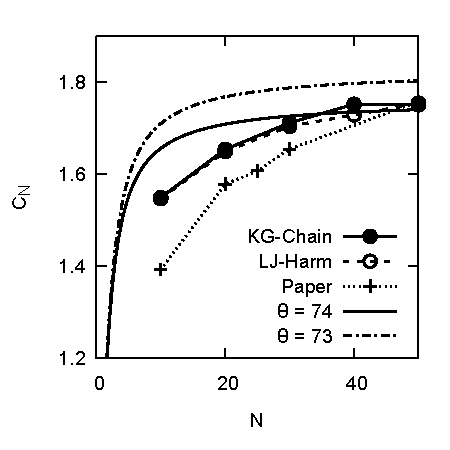
\includegraphics[width=60mm]{./fig/C_ratio.pdf}
	\caption{Characteristic Ratio for varied length of KG Chains and others}
	\label{fig:Characteristic Ratio}
	\end{center}
%\vspace{-10mm}
\end{wrapfigure}

\subsection{鎖の交差}

``KG Chain'' での鎖の交差ポテンシャル $U_{cross} \simeq 70 k_B T$ と見積もれ、通常の条件では鎖の交差が生じないとされる。

非結合ポテンシャル $U_{LJ}(r)$ と線形バネポテンシャル $U_{Harm}$ との組み合わせでは、自然長 $R_0$ とバネ定数 $K$ の適切な設定によりこの値を小さくできる。

\subsection{一軸伸長}
``KG Chain'' からなるダイヤモンドネットワークの一軸伸長($10^{-5}\lambda/\tau$)時の SS カーブを、Fig. \ref{fig: stretch} に示した。


$\lambda<2$ 程度の小さなひずみではネオフッキアンモデルに合致した。
しかし、大変形領域においては、特性比より算出したクーンセグメント数($N_K\simeq 16.6$)に換算した場合には、対応した伸びきり鎖の応力モデル~\cite{Arruda1993}とは合致せず、$N=21$ 程度でフィットできたため、伸長時には平衡状態のアングルから平均的に伸びているものと推測できた。



\begin{wrapfigure}{r}{60mm}
\vspace{-4\baselineskip}
	\begin{center}
	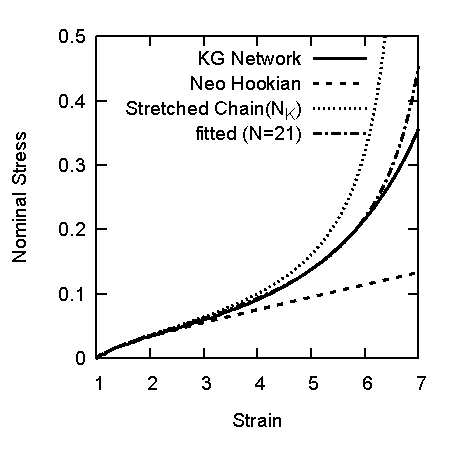
\includegraphics[width=60mm]{./fig/SS.pdf}
	\caption{Uniaxial Elongation SS Curve and Energies Result with Stretched Chain Model~\cite{Arruda1993}}
	\label{fig: stretch}
	\end{center}
%\vspace{-40mm}
\end{wrapfigure}



\bibliographystyle{achemso}
%{elsart-num}
%{junsrt-2}
\bibliography{C:/Dropbox/Tex/TeXworks/library.bib}

\end{document}